\section{Exercise 7.12: Analyzing a Note Played by a Violin} 

% Code listing configuration for MATLAB
\lstset{
    language=Matlab,
    basicstyle=\ttfamily\small,
    keywordstyle=\color{blue},
    stringstyle=\color{purple},
    commentstyle=\color{green!60!black},
    numbers=left,
    numberstyle=\tiny\color{gray},
    breaklines=true,
    frame=single,
    captionpos=b
}

\subsection{MATLAB Implementation}

Below is the MATLAB script \texttt{dft\_unknown\_note.m} written to read the audio recording \texttt{unknown\_note.wav}, calculate its Discrete Fourier Transform (DFT), and plot the magnitude spectrum for the bottom half of the frequency range (from DC up to the Nyquist frequency):

\lstinputlisting[caption={MATLAB script \texttt{dft\_unknown\_note.m}}, label={lst:dft_unknown_note}]{Code/dft_unknown_note.m}

\subsection{Results}

\textbf{Description of the Magnitude Spectrum}

The computed magnitude spectrum $|F(\nu)|$ for \texttt{unknown\_note.wav} exhibits the characteristic acoustic signature of a plucked or bowed string instrument:
\begin{figure}[h]
    \centering
    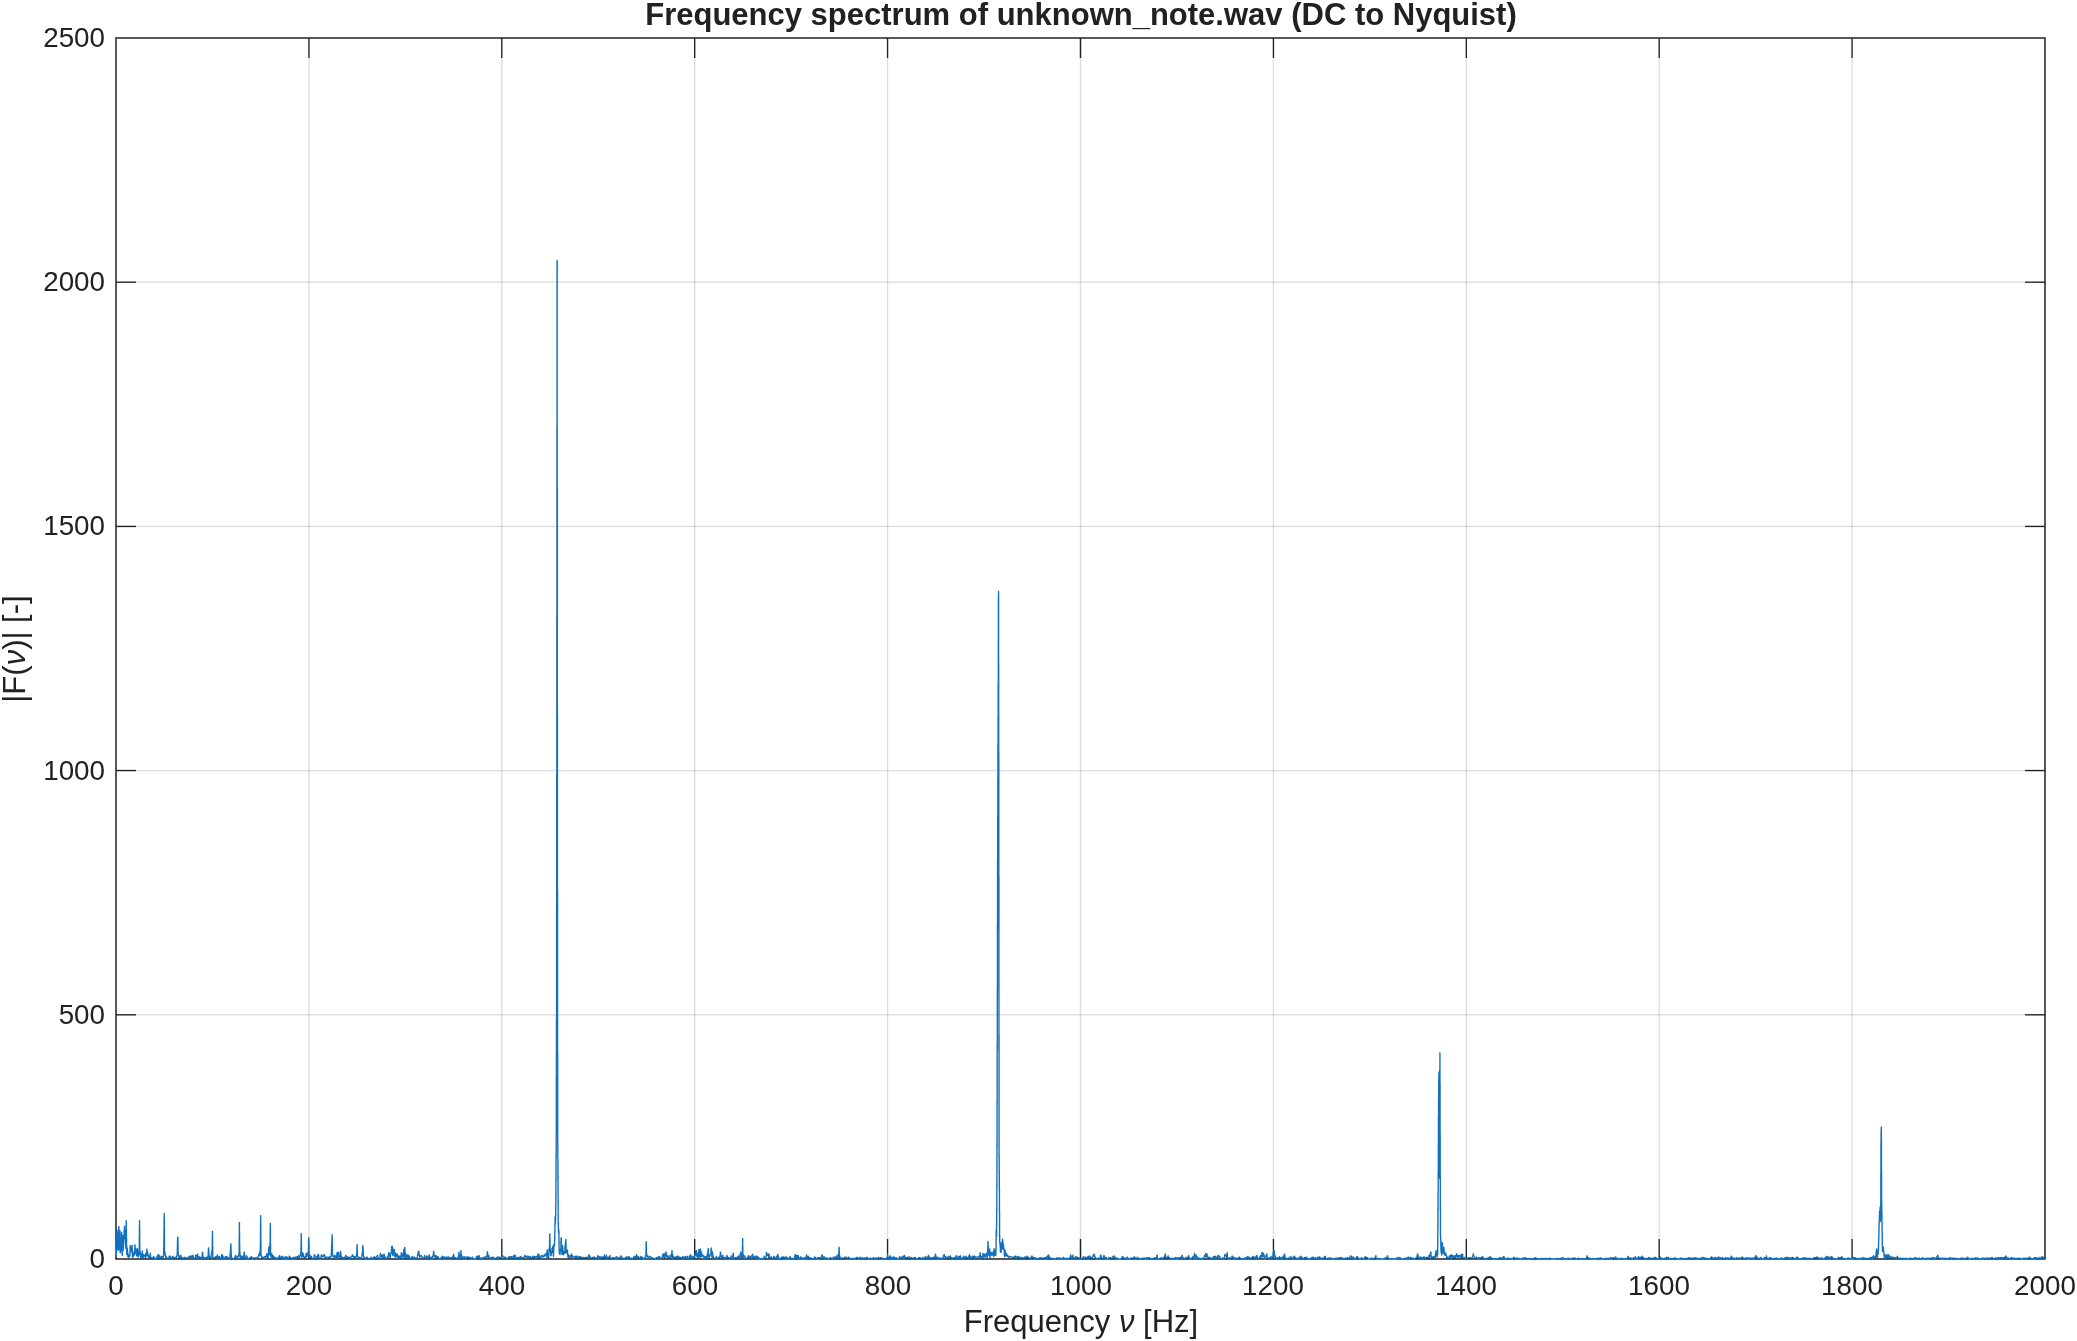
\includegraphics[width=1\linewidth]{Figures/Frequency spectrum for unknown note.png}
    \caption{Frequency spectrum}
    \label{fig:placeholder}
\end{figure}
\begin{itemize}
    \item \textbf{Fundamental Peak:} The sharpest and most prominent peak occurs at approximately $\nu_0 \approx 466.2\text{ Hz}$ with a peak magnitude $|F(\nu)| > 2000$.
    \item \textbf{Harmonic Overtones:} In addition to the base frequency, several distinct secondary peaks appear at integer multiples ($k \cdot \nu_0$) of the fundamental frequency:
    \begin{itemize}
        \item $2^{\text{nd}}$ Harmonic ($2\nu_0$): $\approx 932.3\text{ Hz}$ ($|F(\nu)| \approx 1380$)
        \item $3^{\text{rd}}$ Harmonic ($3\nu_0$): $\approx 1398.5\text{ Hz}$ ($|F(\nu)| \approx 410$)
        \item $4^{\text{th}}$ Harmonic ($4\nu_0$): $\approx 1864.7\text{ Hz}$ ($|F(\nu)| \approx 270$)
    \end{itemize}
    \item \textbf{Noise Level:} The spectral energy between the harmonic peaks is virtually zero, confirming a clean recording with minimal background noise.
\end{itemize}



\pagebreak


\subsection{Results Analysis}
From the peak analysis of the spectrum the Fundamental frequency: 457.35 Hz
\begin{equation}
    \text{Base Frequency } (\nu_0) \approx 466.2\text{ Hz}
\end{equation}

Comparing $\nu_0 = 466.2\text{ Hz}$ against the standard musical note frequency reference table (equal temperament with $\text{A4} = 440.0\text{ Hz}$):
\begin{itemize}
    \item $\text{A4} = 440.00\text{ Hz}$
    \item $\mathbf{A\sharp4 / B\flat4 = 466.16\text{ Hz}}$
    \item $\text{B4} = 493.88\text{ Hz}$
\end{itemize}

\textbf{Conclusion:} The note being played by the violinist in \texttt{unknown\_note.wav} is \textbf{A$\sharp$4} (A-sharp in octave 4) or \textbf{B$\flat$4} (B-flat in octave 4).

% ---- Stray text that was after \end{document} (commented out so it compiles; delete if not needed) ----
% Summary of Key Values in the Solution:Script Name: dft_unknown_note.m1Base Frequency ($\nu_0$): $\approx 466.2 \text{ Hz}$23Identified Note: A♯4 / B♭4 (A-sharp 4 / B-flat 4)3Harmonic Pattern: Decreasing integer multiples near $932 \text{ Hz}$, $1398 \text{ Hz}$, and $1865 \text{ Hz}$ representing the timbre of the violin string
% 1. Fundamental Frequency (Peak Value)Frequency: The primary (tallest) peak is located at approximately 460 Hz (between 400 Hz and 600 Hz, roughly around 455–466 Hz)
% 1.Magnitude: The magnitude $|F(\nu)|$ at this peak reaches just above 20001.2. Overtones / HarmonicsThe plot also clearly displays several harmonic peaks at integer multiples of the fundamental frequency1:2nd Harmonic: Peak near 920 Hz (magnitude ~1380)13rd Harmonic: Peak near 1380 Hz (magnitude ~400)14th Harmonic: Peak near 1840 Hz (magnitude ~270)13. Note IdentificationA fundamental frequency of approximately 460–466 Hz corresponds to A♯4 / B♭4 (A-sharp 4 / B-flat 4) (standard frequency is 466.16 Hz).